\documentclass[border=2mm]{standalone}
\usepackage{mathptmx}            % Times math fonts -- match the paper
\usepackage{amsmath,amssymb,bm}
\usepackage{tikz}
\usetikzlibrary{arrows.meta,calc,decorations.pathreplacing}

\definecolor{bR}{HTML}{E74C3C}
\definecolor{bB}{HTML}{2980B9}
\definecolor{gG}{HTML}{27AE60}
\definecolor{nv}{HTML}{152B4A}
\definecolor{ac}{HTML}{00008C}
\definecolor{mu}{HTML}{AAAAAA}

\newcommand{\vv}[1]{\mathbf{#1}}
\newcommand{\DD}{\vv{D}}
\newcommand{\yy}{\vv{y}}
\newcommand{\xxi}{\boldsymbol{\xi}}

\begin{document}
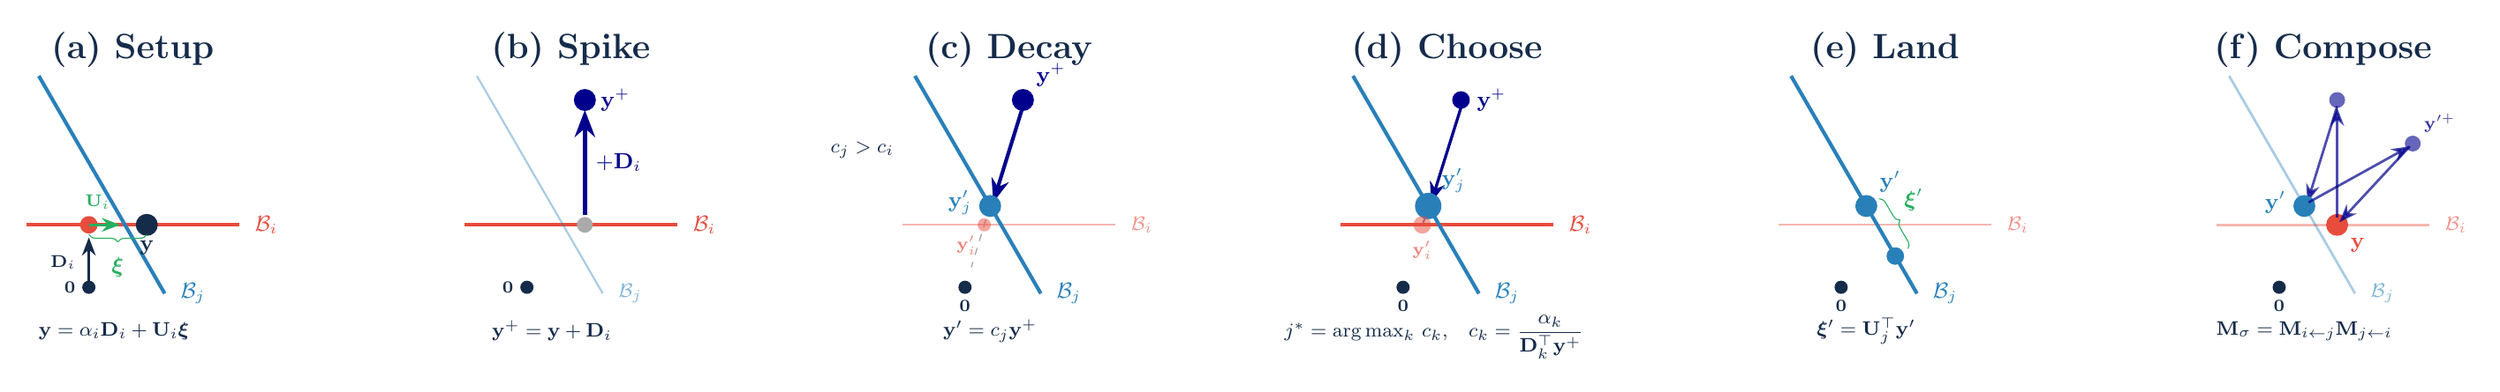
\begin{tikzpicture}[>=Stealth, font=\small, scale=1.8]

% Period-2 (i,j) orbit, theta=60°, alpha_i=alpha_j=0.5
% In SHIFTED coords (B_i at y=0):
%   Origin: (0, -0.5)
%   B_i: y=0 horizontal
%   B_j: y = 0.5 - 1.732 x  (crosses B_i at x=0.289)
%   y on B_i: (0.463, 0)
%   y+:       (0.463, 1.0)
%   y'_j on B_j: (0.201, 0.151)  -- WINNER
%   y'_i loser candidate on B_i: (0.154, 0)
%   y'+: (1.067, 0.651)
%   y'' = y on B_i: (0.463, 0)  -- PERIOD 2 CLOSES

% (a) Setup
\begin{scope}[shift={(0,0)}]
  \node[font=\Large\bfseries, nv] at (0.35, 1.4) {(a) Setup};

  \draw[bR, line width=1.5pt] (-0.5,0) -- (1.2,0);
  \node[bR, font=\small, right=3pt] at (1.2,0) {$\mathcal{B}_i$};
  \draw[bB, line width=1.5pt] (-0.40,1.193) -- (0.606,-0.55);
  \node[bB, font=\small, right=3pt] at (0.606,-0.55) {$\mathcal{B}_j$};

  % Origin
  \fill[nv] (0,-0.5) circle (1.5pt);
  \node[nv, font=\scriptsize, left=2pt] at (0,-0.5) {$\vv{0}$};

  % Foot of B_i
  \fill[bR] (0,0) circle (2pt);

  % D_i arrow from origin toward foot
  \draw[->, nv, line width=1pt] (0,-0.5) -- (0,-0.1);
  \node[nv, font=\scriptsize, left=2pt] at (0,-0.3) {$\DD_i$};

  % U_i arrow from foot along bound (rightward, in same direction as xi)
  \draw[->, gG, line width=1pt] (0,0) -- (0.25,0);
  \node[gG, font=\scriptsize, above=2pt] at (0.07,0.02) {$\vv{U}_i$};

  % y on B_i (label below B_i, kept clear of B_j by sitting at small |y|)
  \fill[nv] (0.463,0) circle (2.5pt);
  \node[nv, font=\small, below=3pt] at (0.463,0) {$\yy$};

  % xi brace -- moved further along pointing direction
  \draw[gG, decorate, decoration={brace, amplitude=3pt, mirror, raise=4pt}]
    (0,0) -- (0.463,0);
  \node[gG, font=\small, below=12pt] at (0.23,0.04) {$\xxi$};

  \node[nv, font=\footnotesize] at (0.2, -0.85) {$\yy = \alpha_i\DD_i + \vv{U}_i\xxi$};
\end{scope}

% (b) Spike
\begin{scope}[shift={(3.5,0)}]
  \node[font=\Large\bfseries, nv] at (0.35, 1.4) {(b) Spike};

  \draw[bR, line width=1.5pt] (-0.5,0) -- (1.2,0);
  \node[bR, font=\small, right=3pt] at (1.2,0) {$\mathcal{B}_i$};
  \draw[bB, line width=0.8pt, opacity=0.4] (-0.40,1.193) -- (0.606,-0.55);
  \node[bB, font=\footnotesize, opacity=0.6, right=3pt] at (0.606,-0.55) {$\mathcal{B}_j$};

  \fill[nv] (0,-0.5) circle (1.5pt);
  \node[nv, font=\scriptsize, left=2pt] at (0,-0.5) {$\vv{0}$};

  \fill[mu] (0.463,0) circle (1.8pt);

  \fill[ac] (0.463,1.0) circle (2.5pt);
  \node[ac, font=\small, right=3pt] at (0.463,1.0) {$\yy^+$};

  \draw[->, ac, line width=1.8pt] (0.463,0.08) -- (0.463,0.92);
  \node[ac, font=\small, right=1pt] at (0.463,0.5) {$+\DD_i$};

  \node[nv, font=\footnotesize] at (0.2, -0.85) {$\yy^+ = \yy + \DD_i$};
\end{scope}

% (c) Decay
\begin{scope}[shift={(7.0,0)}]
  \node[font=\Large\bfseries, nv] at (0.35, 1.4) {(c) Decay};

  \draw[bR, line width=0.8pt, opacity=0.4] (-0.5,0) -- (1.2,0);
  \node[bR, font=\footnotesize, opacity=0.6, right=3pt] at (1.2,0) {$\mathcal{B}_i$};
  \draw[bB, line width=1.5pt] (-0.40,1.193) -- (0.606,-0.55);
  \node[bB, font=\small, right=3pt] at (0.606,-0.55) {$\mathcal{B}_j$};

  \fill[nv] (0,-0.5) circle (1.5pt);
  \node[nv, font=\scriptsize, below=2pt] at (0,-0.5) {$\vv{0}$};

  \fill[ac] (0.463,1.0) circle (2.5pt);
  \node[ac, font=\small, above right=2pt] at (0.463,1.0) {$\yy^+$};

  % Decay arrow y+ -> y'_j
  \draw[->, ac, line width=1.5pt] (0.463,0.95) -- (0.225,0.18);

  % Dashed continuation toward origin
  \draw[mu, dashed, line width=0.5pt] (0.201,0.151) -- (0.05,-0.34);

  \fill[bB] (0.201,0.151) circle (2.5pt);
  \node[bB, font=\small, left=3pt] at (0.18,0.18) {$\yy'_j$};

  \fill[bR, opacity=0.5] (0.154,0) circle (1.5pt);
  \node[bR, opacity=0.7, font=\scriptsize, below left=0pt] at (0.158,-0.02) {$\yy'_i$};

  \node[nv, font=\footnotesize, anchor=east] at (-0.5, 0.6) {$c_j > c_i$};
  \node[nv, font=\footnotesize] at (0.2, -0.85) {$\yy' = c_j\yy^+$};
\end{scope}

% (d) Choose — competing candidates, argmax wins
\begin{scope}[shift={(10.5,0)}]
  \node[font=\Large\bfseries, nv] at (0.35, 1.4) {(d) Choose};

  \draw[bR, line width=1.5pt] (-0.5,0) -- (1.2,0);
  \node[bR, font=\small, right=3pt] at (1.2,0) {$\mathcal{B}_i$};
  \draw[bB, line width=1.5pt] (-0.40,1.193) -- (0.606,-0.55);
  \node[bB, font=\small, right=3pt] at (0.606,-0.55) {$\mathcal{B}_j$};

  \fill[nv] (0,-0.5) circle (1.5pt);
  \node[nv, font=\scriptsize, below=2pt] at (0,-0.5) {$\vv{0}$};

  % y+
  \fill[ac] (0.463,1.0) circle (2pt);
  \node[ac, font=\small, right=3pt] at (0.463,1.0) {$\yy^+$};

  % Decay ray: solid to winner, dashed beyond
  \draw[->, ac, line width=1.2pt] (0.463,0.94) -- (0.225,0.18);
  \draw[ac, dashed, line width=0.8pt, opacity=0.5] (0.225,0.18) -- (0.154,0);

  % Winner on B_j
  \fill[bB] (0.201,0.151) circle (3pt);
  \node[bB, font=\small, above right=2pt] at (0.201,0.151) {$\yy'_j$};

  % Loser on B_i
  \fill[bR, opacity=0.5] (0.154,0) circle (2pt);
  \node[bR, font=\scriptsize, opacity=0.7, below=2pt] at (0.154,-0.02) {$\yy'_i$};

  \node[nv, font=\footnotesize, align=center] at (0.25, -0.90)
    {$j^* = \arg\max_k\, c_k$,\quad $c_k=\dfrac{\alpha_k}{\DD_k^\top\yy^+}$};
\end{scope}

% (e) Land
\begin{scope}[shift={(14.0,0)}]
  \node[font=\Large\bfseries, nv] at (0.35, 1.4) {(e) Land};

  \draw[bR, line width=0.8pt, opacity=0.4] (-0.5,0) -- (1.2,0);
  \node[bR, font=\footnotesize, opacity=0.6, right=3pt] at (1.2,0) {$\mathcal{B}_i$};
  \draw[bB, line width=1.5pt] (-0.40,1.193) -- (0.606,-0.55);
  \node[bB, font=\small, right=3pt] at (0.606,-0.55) {$\mathcal{B}_j$};

  \fill[nv] (0,-0.5) circle (1.5pt);
  \node[nv, font=\scriptsize, below=2pt] at (0,-0.5) {$\vv{0}$};

  % Foot of B_j (perpendicular from origin)
  \fill[bB] (0.433,-0.25) circle (2pt);

  \fill[bB] (0.201,0.151) circle (2.5pt);
  \node[bB, font=\small, above right=2pt] at (0.201,0.151) {$\yy'$};

  \draw[gG, decorate, decoration={brace, amplitude=3pt, mirror, raise=6pt}]
    (0.433,-0.25) -- (0.201,0.151);
  \node[gG, font=\small] at (0.58,0.20) {$\xxi'$};

  \node[nv, font=\footnotesize] at (0.2, -0.85) {$\xxi' = \vv{U}_j^\top\yy'$};
\end{scope}

% (f) Compose — show FULL period-2 trajectory
\begin{scope}[shift={(17.5,0)}]
  \node[font=\Large\bfseries, nv] at (0.35, 1.4) {(f) Compose};

  \draw[bR, line width=1.0pt, opacity=0.4] (-0.5,0) -- (1.2,0);
  \node[bR, font=\footnotesize, opacity=0.6, right=3pt] at (1.2,0) {$\mathcal{B}_i$};
  \draw[bB, line width=1.0pt, opacity=0.4] (-0.40,1.193) -- (0.606,-0.55);
  \node[bB, font=\footnotesize, opacity=0.6, right=3pt] at (0.606,-0.55) {$\mathcal{B}_j$};

  \fill[nv] (0,-0.5) circle (1.5pt);
  \node[nv, font=\scriptsize, below=2pt] at (0,-0.5) {$\vv{0}$};

  % First spike: y at (0.463, 0) -> y+ at (0.463, 1.0)
  \fill[bR] (0.463,0) circle (2.5pt);
  \node[bR, font=\small, below right=2pt] at (0.463,0) {$\yy$};
  \draw[->, ac, line width=1pt, opacity=0.7] (0.463,0.06) -- (0.463,0.94);

  % y+
  \fill[ac, opacity=0.6] (0.463,1.0) circle (1.8pt);

  % First decay: y+ -> y'_j on B_j at (0.201, 0.151)
  \draw[->, ac, line width=1pt, opacity=0.7] (0.463,0.95) -- (0.225,0.18);

  % y' on B_j
  \fill[bB] (0.201,0.151) circle (2.5pt);
  \node[bB, font=\small, left=3pt] at (0.18,0.18) {$\yy'$};

  % Second spike: y' -> y'+ = y' + D_j = (0.201 + 0.866, 0.151 + 0.5) = (1.067, 0.651)
  \draw[->, ac, line width=1pt, opacity=0.7] (0.235,0.18) -- (1.043,0.629);

  % y'+
  \fill[ac, opacity=0.6] (1.067,0.651) circle (1.8pt);
  \node[ac, font=\scriptsize, opacity=0.8, above right=1pt] at (1.07,0.65) {$\yy'^+$};

  % Second decay: y'+ -> y'' at (0.463, 0) -- BACK TO START
  \draw[->, ac, line width=1pt, opacity=0.7] (1.043,0.628) -- (0.480,0.020);

  \node[nv, font=\footnotesize] at (0.2, -0.85) {$\vv{M}_\sigma = \vv{M}_{i\leftarrow j}\vv{M}_{j\leftarrow i}$};
\end{scope}

\end{tikzpicture}
\end{document}
